%%%%%%%%%%%%%%%%%%%%%%%%%%%%%%%%%%%%%%%%%
% Wenneker Assignment
% LaTeX Template
% Version 2.0 (12/1/2019)
%
% This template originates from:
% http://www.LaTeXTemplates.com
%
% Authors:
% Vel (vel@LaTeXTemplates.com)
% Frits Wenneker
%
% License:
% CC BY-NC-SA 3.0 (http://creativecommons.org/licenses/by-nc-sa/3.0/)
% 
%%%%%%%%%%%%%%%%%%%%%%%%%%%%%%%%%%%%%%%%%

%----------------------------file:///home/thiago/Documentos/NLP/TP1/word2vec/trunk/datasets/results.png------------------------------------------------------------
%	PACKAGES AND OTHER DOCUMENT CONFIGURATIONS
%----------------------------------------------------------------------------------------

\documentclass[11pt]{scrartcl} % Font size
\usepackage{float}
\usepackage{hyperref}
\usepackage[dvipsnames]{xcolor}
%%%%%%%%%%%%%%%%%%%%%%%%%%%%%%%%%%%%%%%%%
% Wenneker Assignment
% Structure Specification File
% Version 2.0 (12/1/2019)
%
% This template originates from:
% http://www.LaTeXTemplates.com
%
% Authors:
% Vel (vel@LaTeXTemplates.com)
% Frits Wenneker
%
% License:
% CC BY-NC-SA 3.0 (http://creativecommons.org/licenses/by-nc-sa/3.0/)
% 
%%%%%%%%%%%%%%%%%%%%%%%%%%%%%%%%%%%%%%%%%

%----------------------------------------------------------------------------------------
%	PACKAGES AND OTHER DOCUMENT CONFIGURATIONS
%----------------------------------------------------------------------------------------

\usepackage{amsmath, amsfonts, amsthm} % Math packages

\usepackage{listings} % Code listings, with syntax highlighting

\usepackage[english]{babel} % English language hyphenation

\usepackage{graphicx} % Required for inserting images
\graphicspath{{Figures/}{./}} % Specifies where to look for included images (trailing slash required)

\usepackage{booktabs} % Required for better horizontal rules in tables

\numberwithin{equation}{section} % Number equations within sections (i.e. 1.1, 1.2, 2.1, 2.2 instead of 1, 2, 3, 4)
\numberwithin{figure}{section} % Number figures within sections (i.e. 1.1, 1.2, 2.1, 2.2 instead of 1, 2, 3, 4)
\numberwithin{table}{section} % Number tables within sections (i.e. 1.1, 1.2, 2.1, 2.2 instead of 1, 2, 3, 4)

\setlength\parindent{0pt} % Removes all indentation from paragraphs

\usepackage{enumitem} % Required for list customisation
\setlist{noitemsep} % No spacing between list items

%----------------------------------------------------------------------------------------
%	DOCUMENT MARGINS
%----------------------------------------------------------------------------------------

\usepackage{geometry} % Required for adjusting page dimensions and margins

\geometry{
	paper=a4paper, % Paper size, change to letterpaper for US letter size
	top=2.5cm, % Top margin
	bottom=3cm, % Bottom margin
	left=3cm, % Left margin
	right=3cm, % Right margin
	headheight=0.75cm, % Header height
	footskip=1.5cm, % Space from the bottom margin to the baseline of the footer
	headsep=0.75cm, % Space from the top margin to the baseline of the header
	%showframe, % Uncomment to show how the type block is set on the page
}

%----------------------------------------------------------------------------------------
%	FONTS
%----------------------------------------------------------------------------------------

\usepackage[utf8]{inputenc} % Required for inputting international characters
\usepackage[T1]{fontenc} % Use 8-bit encoding


%----------------------------------------------------------------------------------------
%	SECTION TITLES
%----------------------------------------------------------------------------------------

\usepackage{sectsty} % Allows customising section commands

\sectionfont{\vspace{6pt}\centering\normalfont\scshape} % \section{} styling
\subsectionfont{\normalfont\bfseries} % \subsection{} styling
\subsubsectionfont{\normalfont\itshape} % \subsubsection{} styling
\paragraphfont{\normalfont\scshape} % \paragraph{} styling

%----------------------------------------------------------------------------------------
%	HEADERS AND FOOTERS
%----------------------------------------------------------------------------------------

\usepackage{scrlayer-scrpage} % Required for customising headers and footers

\ohead*{} % Right header
\ihead*{} % Left header
\chead*{} % Centre header

\ofoot*{} % Right footer
\ifoot*{} % Left footer
\cfoot*{\pagemark} % Centre footer
 % Include the file specifying the document structure and custom commands

%----------------------------------------------------------------------------------------
%	TITLE SECTION
%----------------------------------------------------------------------------------------

\title{	
	\normalfont\normalsize
	\textsc{Departamento de Ciência da Computaçao - UFMG}\\ % Your university, school and/or department name(s)
	\vspace{25pt} % Whitespace
	\rule{\linewidth}{0.5pt}\\ % Thin top horizontal rule
	\vspace{20pt} % Whitespace
	{\huge Trabalho Prático II - Aprendizado Profundo para Processamento de Linguagem Natural}\\ % The assignment title
	\vspace{12pt} % Whitespace
	\rule{\linewidth}{2pt}\\ % Thick bottom horizontal rule
	\vspace{12pt} % Whitespace
}

\author{\LARGE Thiago Malta Coutinho\\ thiagomaltac@gmail.com} % Your name

\date{\normalsize\today} % Today's date (\today) or a custom date

\begin{document}



\maketitle % Print the title

%----------------------------------------------------------------------------------------
%	FIGURE EXAMPLE
%----------------------------------------------------------------------------------------

\section{Introdução}

O objetivo desse trabalho prático é estudar a tarefa de POS Tagging, ou classificação gramatical. Nesse estudo uma rede LSTM Bidirecional é implementada para classificar as classes gramaticais do corpus \href{http://nilc.icmc.usp.br/macmorpho/}{Mac-Morpho}, produzido pelo grupo NILC do ICMC-USP. A estrutura do problema e da rede são discutidas assim como a acurácia obtida pelo modelo.

\begin{figure}[h] % [h] forces the figure to be output where it is defined in the code (it suppresses floating)
	\centering
	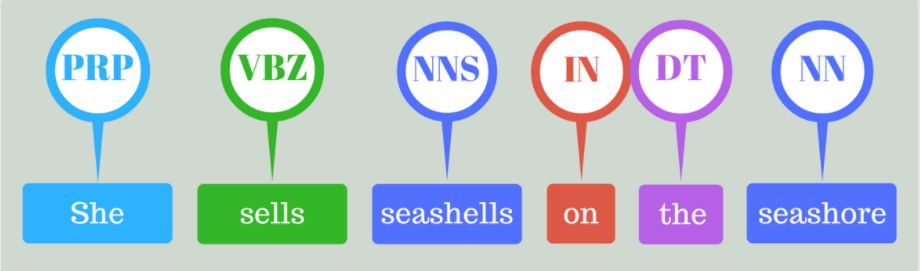
\includegraphics[width=0.8\columnwidth]{./Figures/pos_tagging.png} % Example image
	\caption{Exemplo da tarefa de classificação gramatical, em língua inglesa.}
\end{figure}

%------------------------------------------------

\subsection{Corpus Mac-Morpho}

A descrição da estrutura e das classes presentes no Corpus é feita no Manual, disponível em \href{http://nilc.icmc.usp.br/macmorpho/macmorpho-manual.pdf}{http://nilc.icmc.usp.br/macmorpho/macmorpho-manual.pdf}. No entanto, as classes utilizadas nesse estudo foram definidas pelo método de pré-processamento de dados descrito na Seção \ref{sec:preproc}. Os rótulos e a classe gramatical correspondente são apresentados na Tabela \ref{tab:classes-corpus} abaixo:

\begin{table}[H]
	\centering
	\begin{tabular}{|c|c|}
		\hline
		RÓTULO & CLASSE GRAMATICAL \\ \hline
		N & NOME \\ \hline
		PU & PONTUAÇÃO \\ \hline
		V & VERBO \\ \hline
		NPROP & NOME PRÓPRIO \\ \hline
		PREP & PREPOSIÇÃO \\ \hline
		ART & ARTIGO \\ \hline
		PREP+ART & PREPOSIÇÃO + ARTIGO \\ \hline
		ADJ & ADJETIVO \\ \hline
		ADV & ADVÉRBIO \\ \hline
		KC & CONJUNÇÃO COORDENATIVA \\ \hline
		PCP & PARTICÍPIO \\ \hline
		NUM & NUMERAL \\ \hline
		PROADJ & PRONOME ADJETIVO \\ \hline
		KS & CONJUNÇÃO SUBORDINATIVA \\ \hline
		PRO-KS & \begin{tabular}[c]{@{}c@{}}PRONOME CONECTIVO\\ SUBORDINATIVO\end{tabular} \\ \hline
		PROPESS & PRONOME PESSOAL \\ \hline
		PROSUB & PRONOME SUBSTANTIVO \\ \hline
		PDEN & PALAVRA DENOTATIVA \\ \hline
		CUR & SÍMBOLO DE MOEDA CORRENTE \\ \hline
		PREP+PROADJ & PREPOSIÇÃO + PRONOME ADJETIVO \\ \hline
		ADV-KS & \begin{tabular}[c]{@{}c@{}}ADVÉRBIO CONECTIVO\\ SUBORDINATIVO\end{tabular} \\ \hline
		PREP+PROSUB & PREPOSIÇÃO + PRONOME SUBSTANTIVO \\ \hline
		PREP+PROPESS & PREPOSIÇÃO + PRONOME PESSOAL \\ \hline
		IN & INTERJEIÇÃO \\ \hline
		PREP+PRO-KS & \begin{tabular}[c]{@{}c@{}}PREPOSIÇÃO + \\ PRONOME CONECTIVO\\ SUBORDINATIVO\end{tabular} \\ \hline
		PREP+ADV & PREPOSIÇÃO + ADVÉRBIO \\ \hline
	\end{tabular}
	\caption{Rótulos e Classes gramaticais analisadas no Corpus Mac-Morpho.}
	\label{tab:classes-corpus}
\end{table}


\subsection{LSTM}

\begin{figure}[H] % [h] forces the figure to be output where it is defined in the code (it suppresses floating)
	\centering
	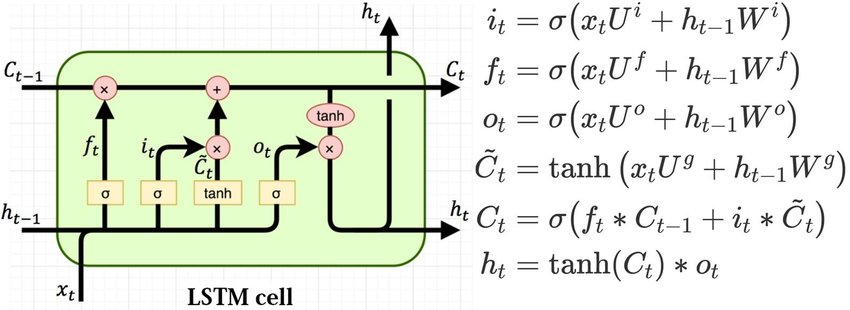
\includegraphics[width=0.7\columnwidth]{./Figures/lstm_and_equations.jpg} % Example image
	\caption{Célula LSTM com as operações internas explicitadas.}
\end{figure}

O modelo LSTM(Long-Short Term Memory) é um modelo que aprende dependências temporais em dados sequenciais. Ele possui representações internas chamadas de estado escondido e célula de memória, que são modificadas de acordo com os dados de entrada e as representações anteriores.

Dentro de cada célula LSTM, os dados de entrada e as representações internas anteriores passam por camadas de transformações lineares seguidas de funções não-lineares como a tangente hiperbólica(tanh) e a função sigmoide($\sigma$). Para controlar o fluxo de dados ao longo do tempo, existem três \textit{gates}: $i_{t}$, que controla o quanto de informação entra na célula; $f_{t}$ controla o quanto o estado de memória anterior será suavizado, ou "esquecido"; $o_{t}$ limita o quanto de informação interna da célula atual será transferida para o estado escondido atual. Além dos \textit{gates} existem duas transformações não-lineares dentro da célula: $\tilde{C}_{t}$, uma representação intermediária da célula memória atual; e $h_{t}$ que é o novo estado escondido.

\begin{figure}[H] % [h] forces the figure to be output where it is defined in the code (it suppresses floating)
	\centering
	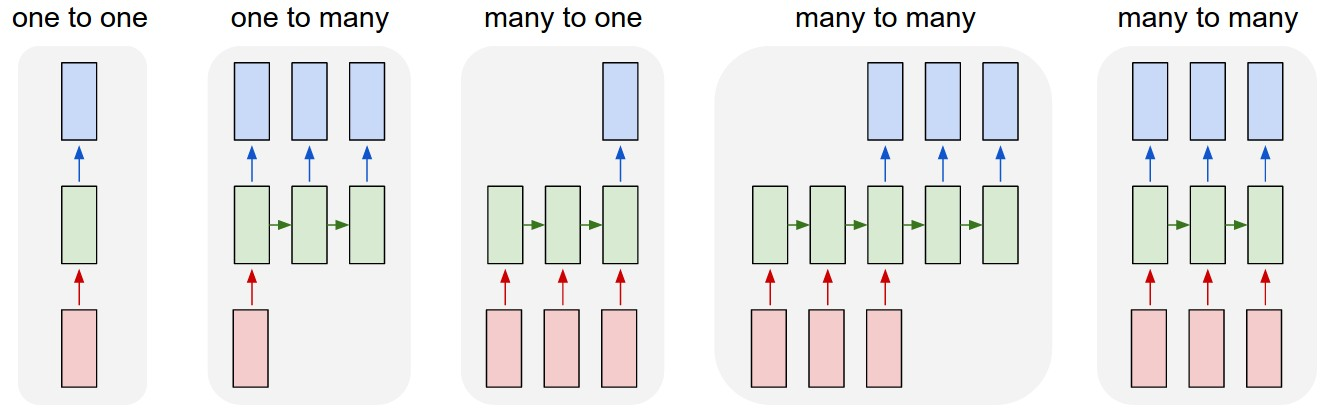
\includegraphics[width=0.8\columnwidth]{./Figures/lstm_usages.jpeg} % Example image
	\caption{Exemplos de diferentes usos da arquitetura LSTM.}
	\label{fig:lstmConfigs}
\end{figure}

A arquitetura da rede neural LSTM pode ser utilizada de diversas maneiras, a Figura \ref{fig:lstmConfigs} exemplifica as configurações mais comuns. Para o problema de \textit{POS Tagging} a organização utilizada é a \textit{Many-to-many} com uma saída para cada entrada, pois para cada palavra deverá ser classificada gramaticalmente.

Cada palavra da frase é representada em um vetor, \textit{one-hot} ou \textit{Embedding}, esse vetor passa pelas transformações da célula LSTM gerando um estado escondido para a palavra atual. O estado escondido passa por uma transformação linear gerando um vetor do tamanho do número de classes gramaticais. A função \textit{Softmax} é aplicada sobre o vetor para gerar probabilidades de ocorrêcia de cada classe, a classe com maior probabilidade será atribuída a palavra atual. 

É importante ressaltar que cada vetor de probabilidades gerado pela rede LSTM é um vetor de probabilidades condicionais, dado que todas as transformações aplicadas na entrada atual são condicionadas pelo estado escondido anterior e a célula de memória anterior.

Os pesos da rede são atualizados utilizando o BPTT(Back propagation through time) e uma função de custo, como a entropia cruzada, por exemplo.

\subsection{LSTM Bidirecional}
	
\begin{figure}[H] % [h] forces the figure to be output where it is defined in the code (it suppresses floating)
	\centering
	\includegraphics[width=0.7\columnwidth]{./Figures/bilstm.png} % Example image
	\caption{Arquitetura LSTM Bidirecional.}
	\label{fig:bilstm}
\end{figure}
	
A rede LSTM processa os dados em apenas um sentido e isso pode gerar limitações nas representações geradas pelo modelo. Diversos problemas dependem de características presentes em dados mais a frente na sequencia, e percorrer os dados em apenas um sentido não captura essa informação. Uma das soluções possíveis para o problema é instanciar outra rede que percorrerá os dados no sentido contrário, possibilitando representações bidirecionais. Os estados escondidos, ou saídas, de cada rede são concatenados antes de entrarem na camada de transformações lineares que antecede a função \textit{Softmax}. Com essa mudança mais informações podem ser aprendidas dos dados.
	
\section{Experimento}

O experimento consiste no treinamento de uma rede LSTM Bidirecional no conjuntos de dados de treinamento do Corpus Mac-Morpho e avaliação da acurácia do algoritmo no conjunto de teste do Corpus. Para o processamento e projeto da arquitetura foi utilizado o Framework \href{https://pytorch.org/}{PyTorch}, em linguagem Python.

\subsection{Pré-processamento dos dados}\label{sec:preproc}

O pré-processamento dos dados foi feito no conjunto de treinamento e teste. Os dados foram carregados para a memória e as palavras foram separadas das classes correspondentes. A partir dos vetores de palavras e classes um arquivo de dados Tabulares foi gerado para ser processado pelo módulo \texttt{torchtext}, do framework PyTorch. Os dados de treinamento foram dividos em conjunto de treinamento e validação, em uma proporção de 90\% para treino e 10\% validação. 

Utilizando o \texttt{torchtext} \textit{batches} de tamanho 64 foram criados ordenados em ordem decrescente de tamanho para otimização do \textit{padding} dentro da rede neural.


\subsection{Word Embedding}

Semantic Word embeddings são vetores que representam as palavras de forma densa. Eles carregam informações sintáticas e semânticas através do contexto próximo a palavra. Um Word Embedding que se tornou famoso por sua eficácia é o Word2Vec, que existe em duas versões: Skip-gram e CBOW.

Para alimentar a rede um modelo de Word Embedding Word2Vec Skip-gram pré-treinado foi baixado do \href{http://nilc.icmc.usp.br/embeddings}{Repositório de Word Embeddings do NILC}. O modelo possui dimensão 100 e produz representação de entrada melhor que o \textit{one-hot encodding}.

\subsection{Estrutura da rede e hiperparâmetros}

A rede é constituída por uma camada de Embedding, que recebe o Word2Vec 100D pré treinado. Em seguida existem duas camadas de LSTM Bidirecional com uma camada de \texttt{Dropout} ao final das camadas da LSTM, afim de regularizar a rede. Após a cada de \texttt{Dropout} tem uma camada Linear seguida de uma função \textit{Softmax}. O otimizador utilizado foi o Adam, com regularização L2 na atualização dos pesos. Foi aplicado \textit{Gradient Clipping} de norma 6 para evitar \textit{Exploding Gradient}. A dimensão escolhida para o estado escondido foi 100. 

A função de perda utilizada foi a Entropia Cruzada.

\subsection{Rotina de treinamento e avaliação}

A rotina de treinamento consiste em 40 épocas sem atualização dos pesos do Embedding. Isso porque a rede é inicializada com pesos aleatórios e o gradiente pode atualizar a camada de Embedding de forma a piorar sua representação. Nas primeiras 40 épocas a probabilidade da camada de \texttt{Dropout} é igual à 0,25. Após as 40 épocas o algoritmo é treinado por mais 40 épocas mas com atualização dos pesos da camada de Embedding. A probabilidade da camada \texttt{Dropout} é atualizada para 0,4. O aumento da probabilidade se deve ao aumento do número de pesos a serem treinados, mais conexões são podadas afim de evitar o \textit{Overfitting} da rede.


\section{Resultados}

Ao final das 80 épocas de treinamento o modelo foi avaliado no conjunto de teste do Corpus. A acurácia total obtida foi \textbf{91,95\%}.


\begin{figure}[H] % [h] forces the figure to be output where it is defined in the code (it suppresses floating)
	\centering
	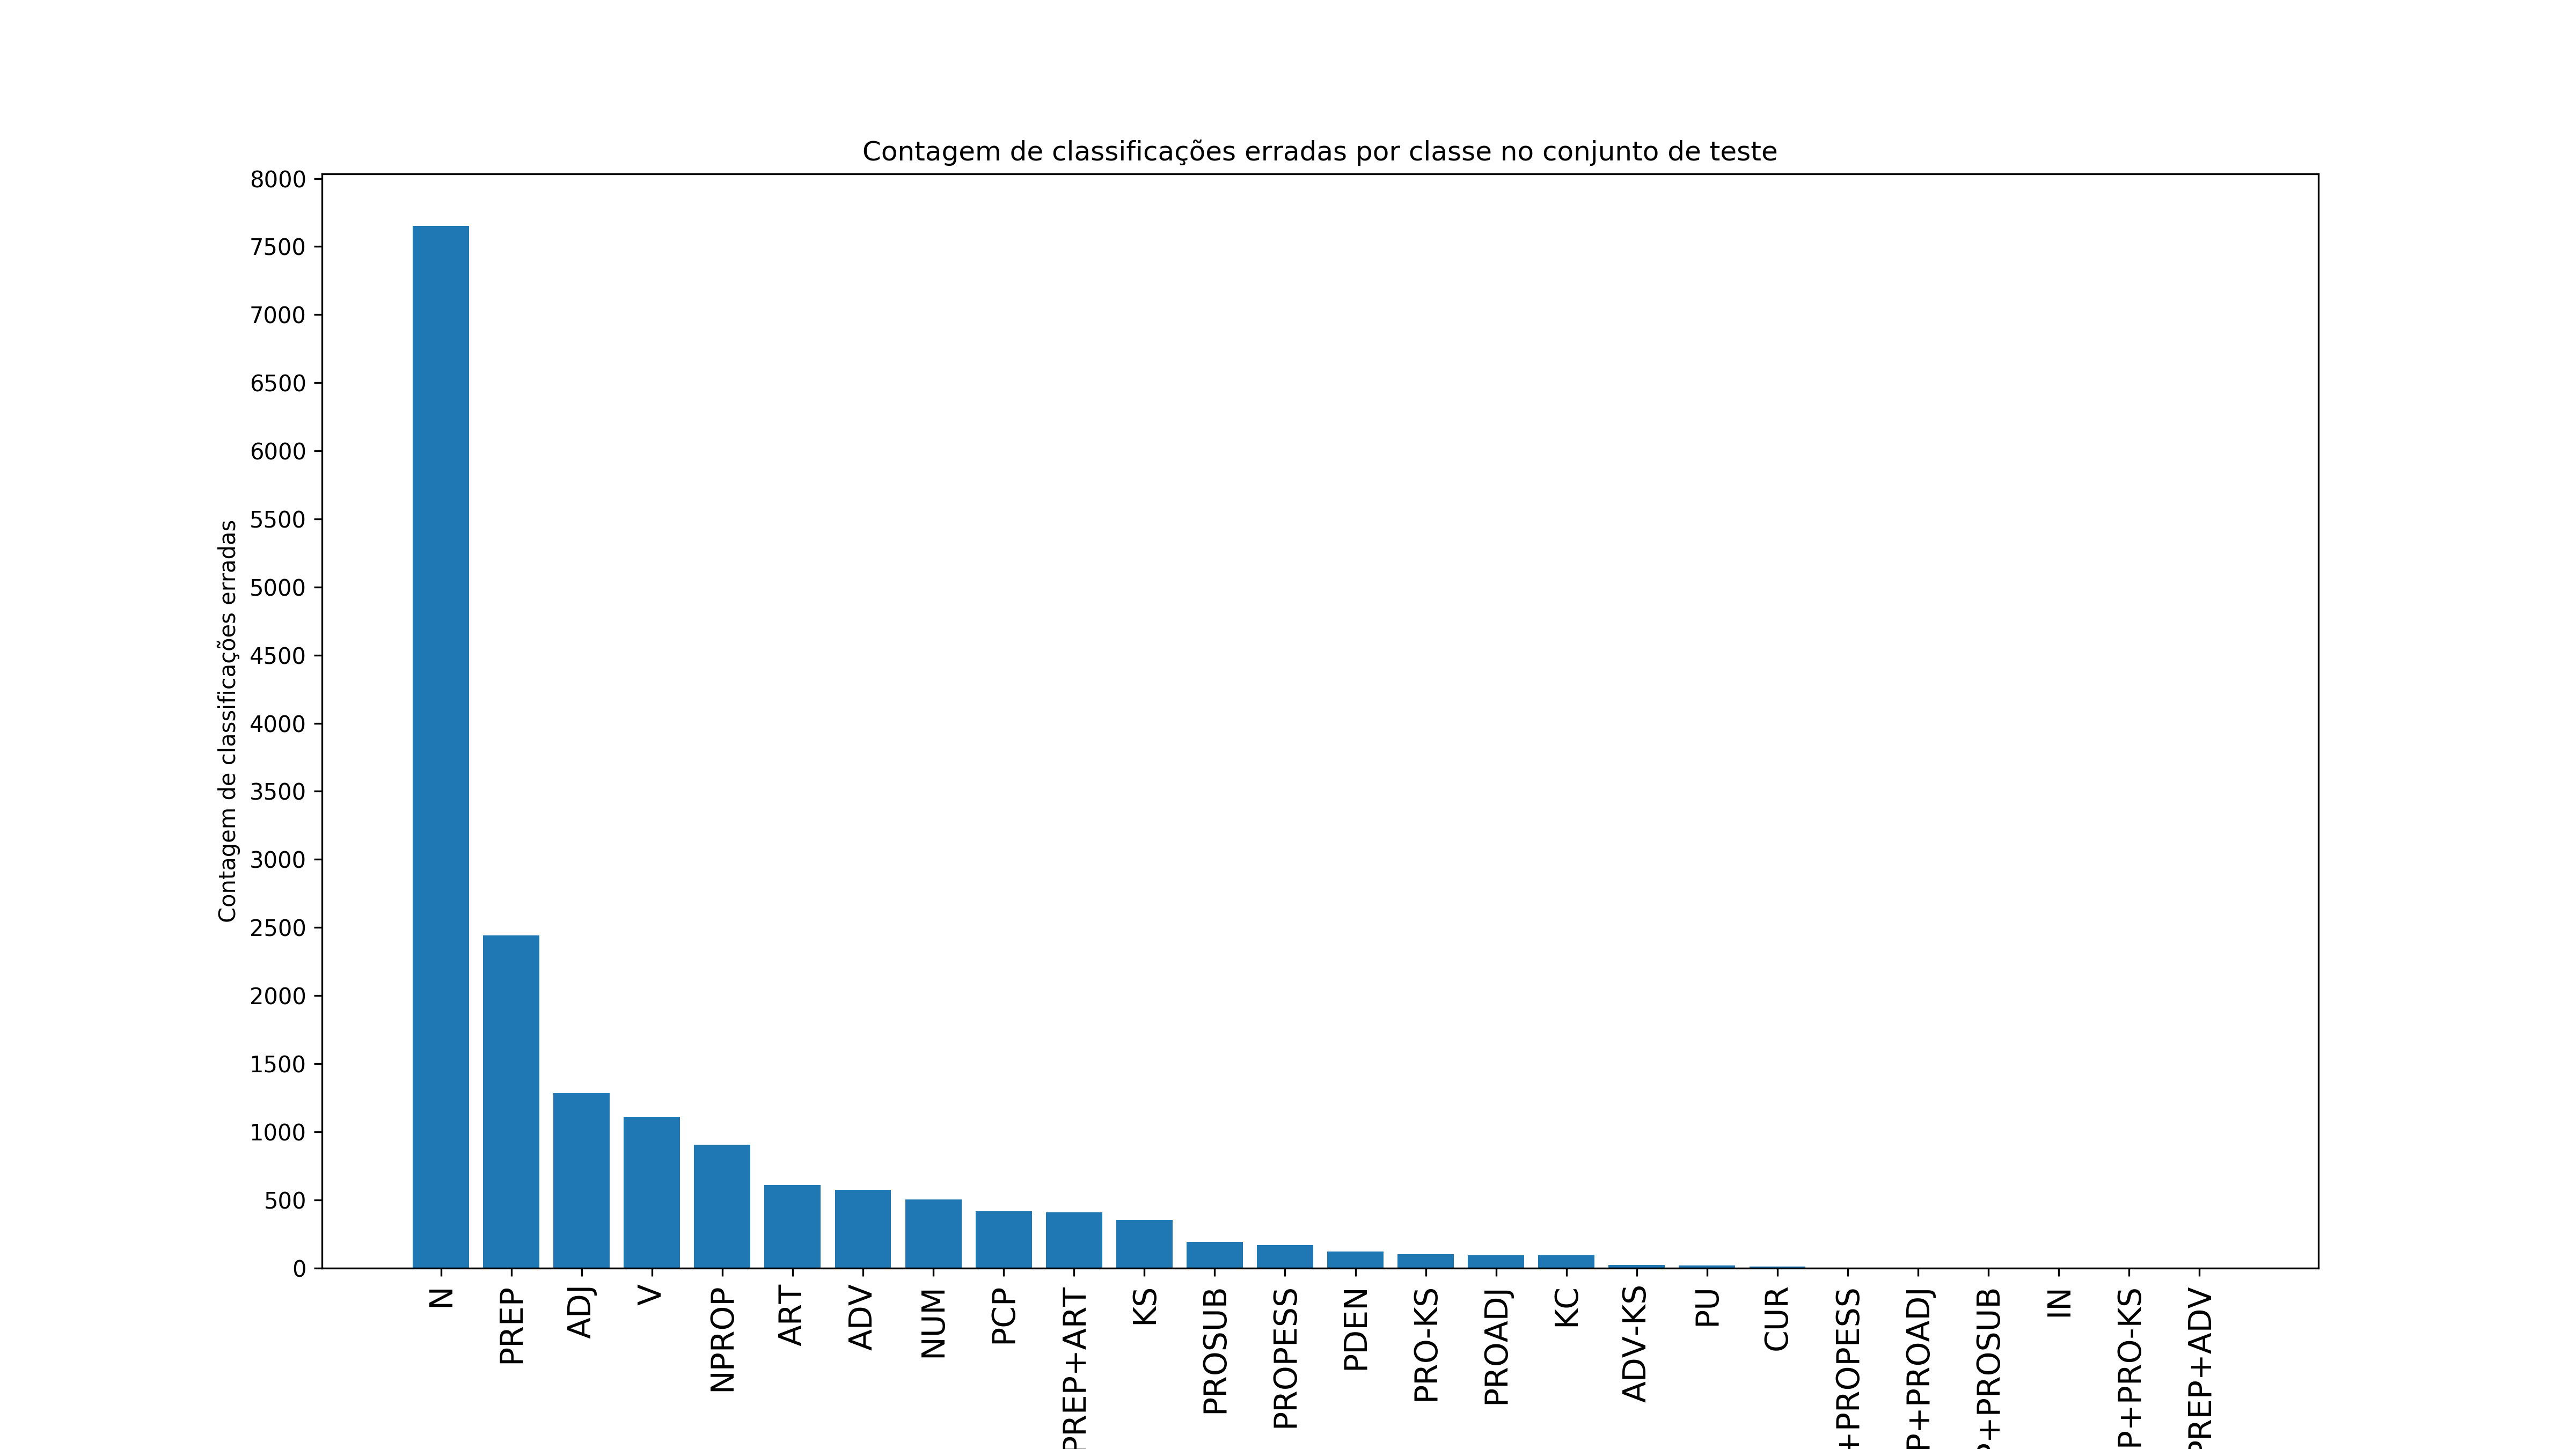
\includegraphics[width=1\columnwidth]{./Figures/contagem_class.png} % Example image
	\caption{Contagem de classificações erradas por classe no conjunto de teste}
	\label{fig:contagem}
\end{figure}

Para avaliar a acurácia do modelo, a contagem de erros por classe foi feita para visualização da quantidade de erros em cada classe.

Como cada classe tem número de ocorrências distinto, a contagem em si não fornece resultados conclusivos. A acurácia por classe foi avaliada para levar em consideração o número de amostras de cada classe.

\begin{figure}[H] % [h] forces the figure to be output where it is defined in the code (it suppresses floating)
	\centering
	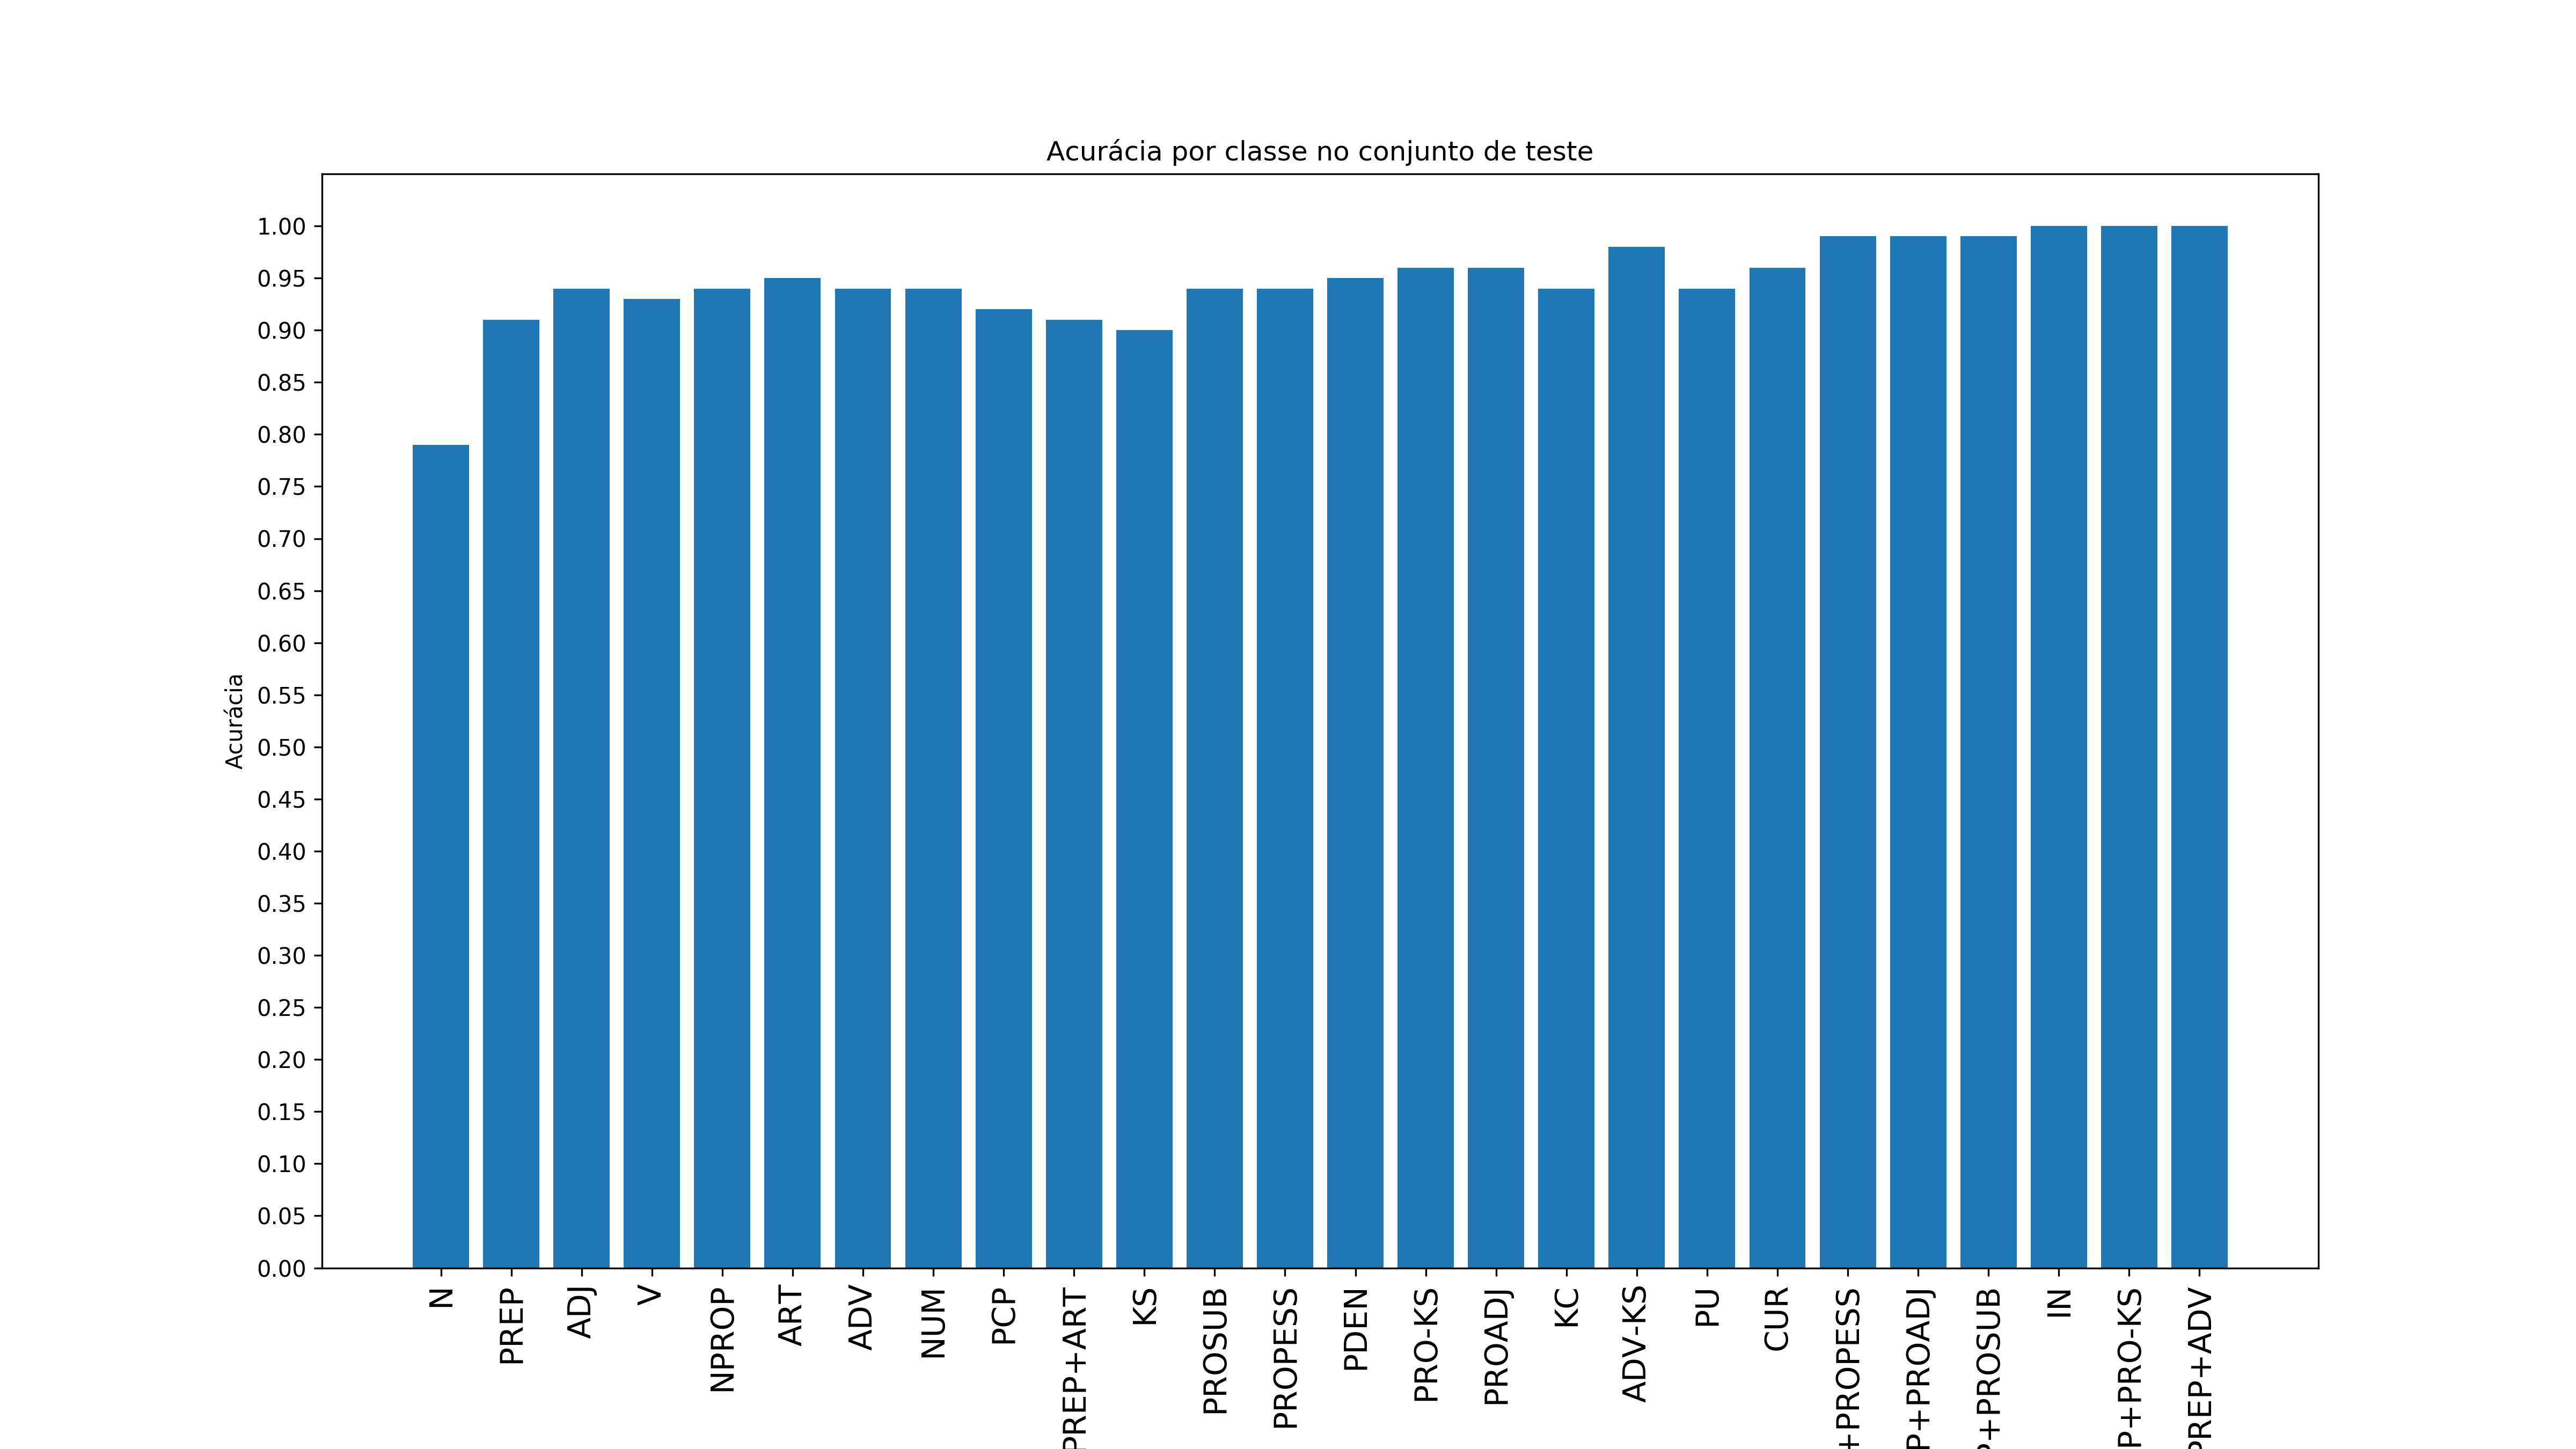
\includegraphics[width=1\columnwidth]{./Figures/acc_class.png} % Example image
	\caption{Acurácia por classe no conjunto de teste}
	\label{fig:acc}
\end{figure}

A partir da Figura \ref{fig:acc}, é possível verificar o comportamento observado na Figura \ref{fig:contagem} tem correlação com a acurácia por classe. A discrepância entre as classes diminuiu ao avaliar a acurácia mas mesmo assim as classes que erraram mais também possuem acurácia menor, em média.


\begin{figure}[H] % [h] forces the figure to be output where it is defined in the code (it suppresses floating)
	\centering
	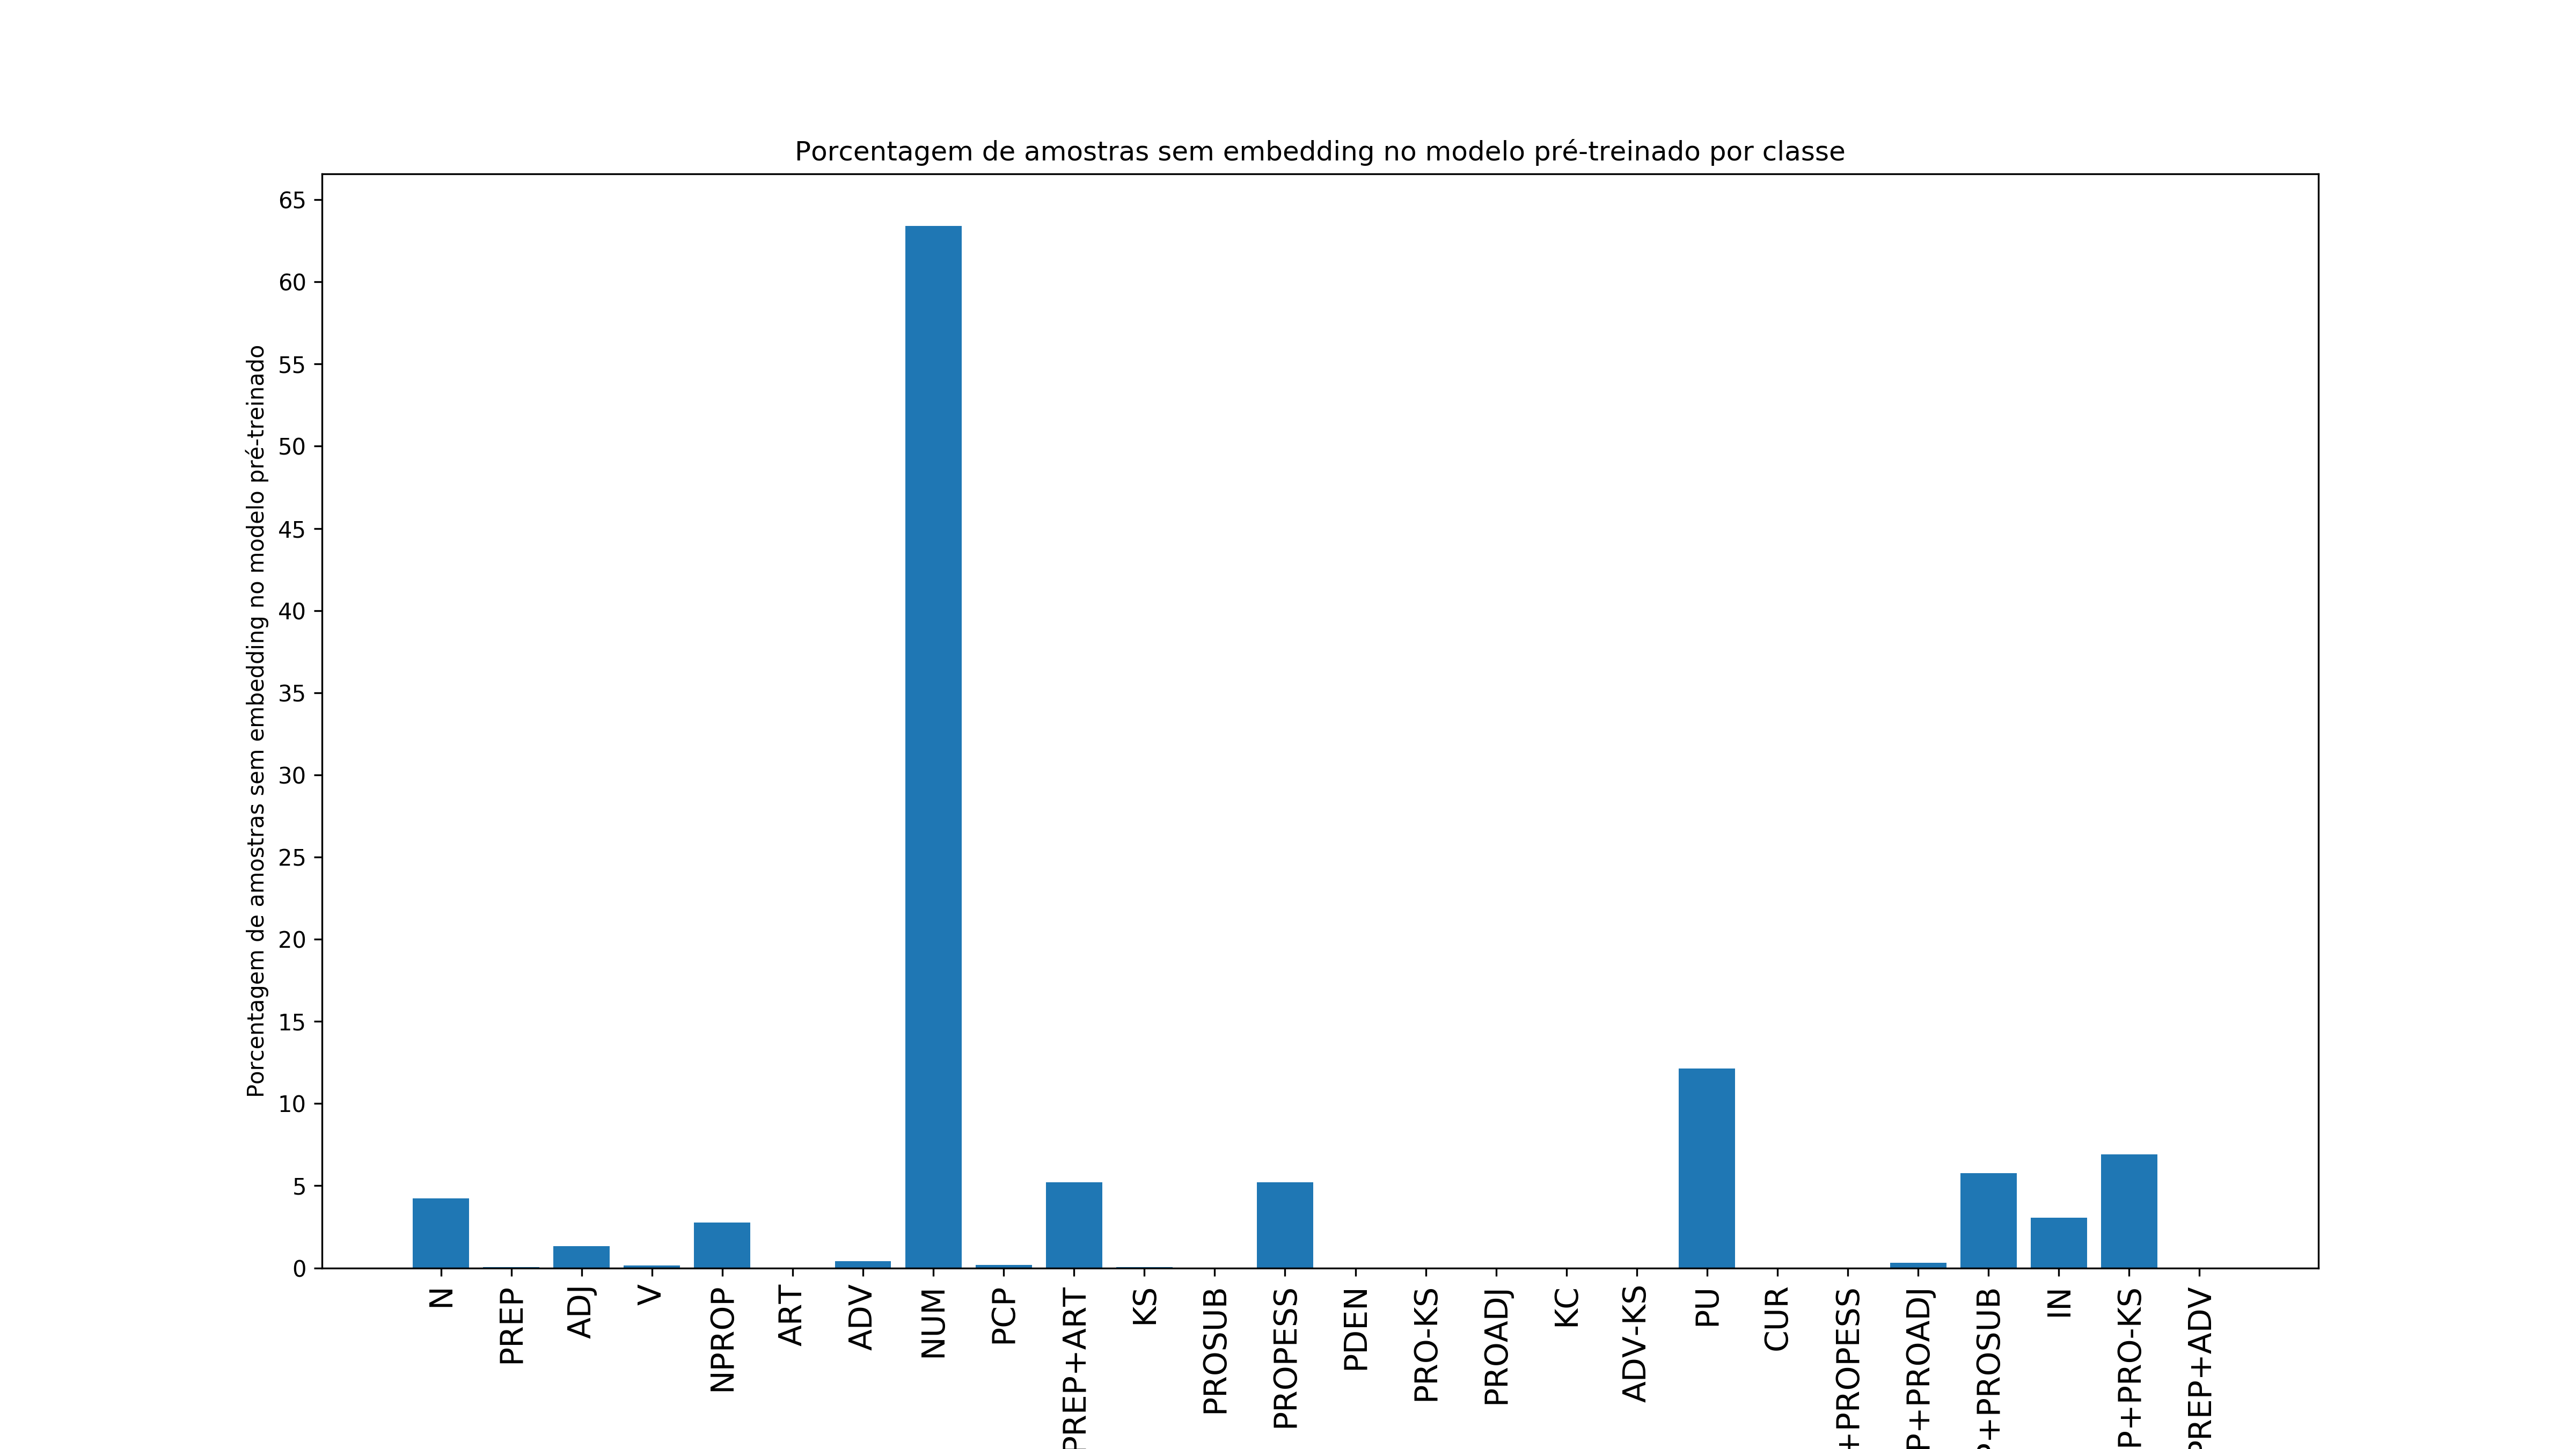
\includegraphics[width=1\columnwidth]{./Figures/perc_embedd.png} % Example image
	\caption{Porcentagem de amostras sem embedding no modelo pré-treinado, por classe}
	\label{fig:embedd}
\end{figure}

Partindo dessa observação, uma hipótese levantada foi a de que a classe de \textbf{Nomes(N)} possui muitos elementos e pode não estar sendo representada corretamente pelo Word2Vec pré-treinado. Foi verificado a porcentagem de palavras que existiam vetores pré-treinados no Word Embedding, os resultados separados por classe estão na Figura \ref{fig:embedd}. Os resultados apontam que boa parte das palavras estavam representadas no Embedding. É possível que se todas as palavras do vocabulário de teste estivessem representadas no Embedding os resultados fossem ligeiramente melhores.

\section{Conclusões}

Esse trabalho estudou o problema de POS Tagging. Nele foi implementado um modelo de aprendizado de máquina baseado na LSTM Bidirecional para classificação gramatical no Corpus Mac-Morpho. 

O modelo foi treinado e obteve resultados satisfatórios, alcançando acurácia geral de \textbf{91,95\%}. Ao observar as acurácias por classe, o modelo deixa a desejar na classe \textbf{Nome(N)}. Um estudo para verificar se existiam representações de Embedding para essa classe e não foi encontrado falta de representação significativa. 

O resultado final pode ser devido à própria arquitetura do modelo e não os dados, mas um estudo mais aprofundado deve ser feito para formar conclusões. Uma melhoria a ser feita no modelo é adicionar uma representação dos caracteres, trazendo mais informação para a classificação. 

Nesse trabalho foi possível estudar o modelo de linguagem \textit{Word2Vec} e entender melhor seu funcionamento. O aluno se familiarizou com a implementação fornecida pelo professor e apresentou uma rotina de avaliação do algoritmo ao variar os parâmetros especificados.


\section{Referências}

1 - Notas de Aula do Professor Adriano Veloso, disciplina de Aprendizado Profundo para Processamento de Linguagem Natural.

2 - \href{https://medium.com/@raghavaggarwal0089/bi-lstm-bc3d68da8bd0}{https://medium.com/@raghavaggarwal0089/bi-lstm-bc3d68da8bd0}

3 - \href{https://pytorch.org/}{https://pytorch.org/}

4 - \href{https://torchtext.readthedocs.io/en/latest/}{https://torchtext.readthedocs.io/en/latest/}

5- \href{https://www.researchgate.net/publication/306093394\_Multilingual\_Part-of-Speech\_Tagging\_with\_Bidirectional\_Long\_Short-Term_Memory\_Models\_and\_Auxiliary_Loss}{https://www.researchgate.net/publication/306093394\_Multilingual\_Part-of-Speech\_Tagging\_with\_Bidirectional\_Long\_Short-Term\_Memory\_Models\_and\_Auxiliary\_Loss}
\end{document}
